% !TEX program = xelatex
\documentclass[UTF8,11pt,fontset=none]{ctexart}
% Use the TeX-distributed AR PL SungtiL GB TrueType font.
% TrueType embedding avoids external Adobe-GB1 CMap rendering dependencies.
% A bare filename also works inside the editor compiler sandbox.
\setCJKmainfont[Script=Default,AutoFakeBold=2,AutoFakeSlant=0.2]{gbsn00lp.ttf}
\setCJKsansfont[Script=Default,AutoFakeBold=2]{gbsn00lp.ttf}
\setCJKmonofont[Script=Default,AutoFakeBold=2]{gbsn00lp.ttf}
\usepackage[a4paper,margin=2.4cm]{geometry}
\usepackage{amsmath,amssymb,booktabs,array,enumitem,xcolor,tikz,listings}
\usepackage[skins,breakable]{tcolorbox}
\usepackage{graphicx,needspace}
\usetikzlibrary{arrows.meta,positioning}
\usepackage{hyperref}
\definecolor{caramel}{HTML}{A9713C}
\definecolor{rosec}{HTML}{D8678F}
\definecolor{paper}{HTML}{FBF4EA}
\definecolor{inkc}{HTML}{3B2E24}
\hypersetup{colorlinks=true,linkcolor=caramel,urlcolor=rosec,
 pdftitle={相遇之后：传染病与种群相互作用，从 SIR 到 Lotka-Volterra},pdfauthor={GPT}}
\linespread{1.08}
\setlength{\parskip}{0.25em}
\setlist{itemsep=0.15em,topsep=0.3em}
\newtcolorbox{keybox}[1][小结]{breakable,enhanced,colback=paper,colframe=caramel,
 boxrule=0.7pt,arc=1.5mm,left=3mm,right=3mm,top=2mm,bottom=2mm,
 title={\bfseries #1},coltitle=white,colbacktitle=caramel,fonttitle=\bfseries}
\newtcolorbox{warnbox}[1][注意]{enhanced,colback=rosec!6,colframe=rosec,
 boxrule=0.7pt,arc=1.5mm,left=3mm,right=3mm,top=2mm,bottom=2mm,
 title={\bfseries #1},coltitle=white,colbacktitle=rosec,fonttitle=\bfseries}
\lstset{language=Python,basicstyle=\ttfamily\footnotesize,
 keywordstyle=\color{caramel}\bfseries,commentstyle=\color{inkc!65},
 stringstyle=\color{rosec},breaklines=true,columns=fullflexible,
 keepspaces=true,showstringspaces=false,frame=single,rulecolor=\color{caramel!50},
 backgroundcolor=\color{paper},aboveskip=0.8em,belowskip=0.8em}
\title{\bfseries 相遇之后：传染病与种群相互作用\\[0.35em]
\large 从 SIR 到 Lotka--Volterra 的微分方程模型}
\author{数学建模笔记}
\date{2026 年 10 月}
\begin{document}
\maketitle\pagestyle{plain}\thispagestyle{empty}
\begin{keybox}[这篇文章想做的事]
一个有传染性的人遇到一个易感者，可能多出一个感染者；
一只捕食者遇到一只猎物，可能少掉一只猎物。
看起来是两件相距很远的事，写成数学后，却都会出现“两个数量相乘”的项。

这篇文章把传染病模型和 Lotka--Volterra 相互作用模型放在一起讲。
后者不只有捕食，还包括争夺资源的竞争、彼此帮助的互利合作。
先从箭头和数量收支建立方程，再看传播阈值、疫情峰值，以及种群的振荡、共存与排斥，最后用矩阵和特征值简要推广到多物种。
\textbf{不要求预先学过微积分}：进阶推导会标出来，可以先读图和文字。
所有参数都是为说明数学而设的假想值，不对应某种疾病或某个真实生态系统。
（本文由 GPT 写作）
\end{keybox}

\section{先认识一种共同的语言：数量怎么变}
用 $X(t)$ 表示时刻 $t$ 的某个数量，$\dot X$ 或 $\mathrm dX/\mathrm dt$
都表示“此刻数量变化得多快”。若单位是人、时间是天，变化速度的单位就是人/天。
\[
\text{数量的变化速度}=\text{进入的速度}-\text{离开的速度}.
\]
微分方程是在规定这个速度，而不是直接给出下一天的数量。
若此刻速度为每天 $2$ 人，不能不加检查地说十天后一定多 $20$ 人，因为中间速度可能改变。

假设两类对象充分混合，数量分别为 $X,Y$。
如果一类数量翻倍，另一类不变，潜在相遇通常也会增多；
最简单的近似是让相遇的贡献与 $XY$ 成正比。
这叫\textbf{双线性交互项}：固定其中一个量时，它对另一个量是一次的。

不过，乘积只是描述相遇的一个理想化起点。
固定每天接触次数的人群，与固定空间里按密度碰面的动物，归一化方式可以不同；
家庭、班级、领地和食物饱和也都可能使这种乘积关系失效。

\section{传染病：先把人群分进三个格子}
基础 \textbf{SIR 模型}把一群人按当前状态分为三类：
\begin{itemize}
\item $S(t)$：易感者，尚可被感染；
\item $I(t)$：有传染性的人，能继续把病原体传给易感者；
\item $R(t)$：已移出传播链的人，在这个基础模型里不再变回易感者。
\end{itemize}
这里的 $I$ 不等于“所有曾经感染过的人”，也不等于每天报告的新增病例。
$R$ 可以代表感染后不再传播且保持免疫的人；
若用它表示其他移出方式，也必须确保该方式真的符合“不再进入传播链”的假设。

\begin{center}
\begin{tikzpicture}[box/.style={draw=caramel,rounded corners=2pt,fill=paper,
 minimum width=2.2cm,minimum height=1.05cm,align=center},>=Stealth]
\node[box] (S) {$S$\\易感};
\node[box,right=2cm of S] (I) {$I$\\有传染性};
\node[box,right=2cm of I] (R) {$R$\\移出};
\draw[->,thick,caramel] (S)--node[above,font=\small] {$\beta SI/N$} (I);
\draw[->,thick,rosec] (I)--node[above,font=\small] {$\gamma I$} (R);
\end{tikzpicture}
\end{center}
箭头上的式子表示\emph{每单位时间的流动量}。
这三个格子也叫\textbf{仓室}，所以 SIR 是一种仓室模型。

先作几条明确假设：观察期内不计出生、迁入迁出；总人数 $N=S+I+R$ 固定；
人群充分混合；进入 $R$ 后不再感染；传播和移出参数暂时不随时间变化。
我们还暂不设置“已经感染但尚无传染性”的中间阶段。
这些不是自然界的通用事实，而是这个版本模型的边界。

\section{两根箭头，怎样写成三个方程}
\subsection{为什么新增感染速度里有一个除以总人数}
设每个有传染性的人，平均每单位时间产生 $\beta$ 次
“若碰到易感者便可导致感染”的有效接触。
充分混合时，接触对象是易感者的比例约为 $S/N$，所以一名传染者带来的新增速度约为
$\beta S/N$。再乘传染者人数 $I$，得到
\[
\text{新增感染速度}=\beta\frac SN I.
\]
若把“接触频率”与“单次传播概率”分开，$\beta$ 可以粗略理解成二者的乘积。
它不仅取决于病原体，也取决于接触环境和行为。
本写法中 $\beta$ 的单位是 $1/\text{天}$；并不是一个无单位的概率。

再设每个传染者以恒定的单位时间速率 $\gamma$ 移出，移出总速度就是 $\gamma I$。
因此
\begin{equation}\label{eq:sir}
\boxed{\begin{aligned}
\dot S&=-\beta SI/N,\\
\dot I&=\beta SI/N-\gamma I,\\
\dot R&=\gamma I.
\end{aligned}}
\end{equation}
每次感染只把一个人从 $S$ 挪到 $I$，每次移出只把一个人从 $I$ 挪到 $R$。
三式相加，右边全部抵消，得到 $\dot S+\dot I+\dot R=0$：
\textbf{分组人数在变，三组之和不变}。

\begin{warnbox}[平均十天，不是每个人恰好十天]
恒定移出速率 $\gamma$ 对应指数分布的传染持续时间，平均长度为 $1/\gamma$。
例如 $\gamma=0.1/\text{天}$，平均持续十天，但模型并没有规定每个人第十天同时移出。
若传染时长具有不同分布，尤其存在明显的固定延迟，需要调整模型结构。
\end{warnbox}

\subsection{一个可以手算开头的假想例子}
令
\[
N=10000,\quad S(0)=9990,\quad I(0)=10,\quad R(0)=0,
\qquad \beta=0.3,\quad\gamma=0.1,
\]
时间单位为天。最开始，新增感染速度为
$0.3\times9990\times10/10000=2.997$ 人/天，移出速度为 $1$ 人/天。
所以 $\dot I(0)=1.997$ 人/天。
这是连续模型在起点的\emph{速度}，不是预测下一天恰好出现 $1.997$ 个新病例。
人口较大时用连续数量近似整体趋势，人数很少时还需要考虑随机事件。

\section{会不会先增长：再生数是一条阈值}
把传染者方程整理成
\[
\dot I=\gamma I\left(\frac\beta\gamma\frac SN-1\right).
\]
只要 $I>0$，它的正负由括号决定。
在几乎全体易感的条件下，一名传染者每单位时间带来约 $\beta$ 个新感染，
持续时间平均为 $1/\gamma$，所以本模型的\textbf{基本再生数}为
\[
\boxed{\mathcal R_0=\frac\beta\gamma.}
\]
它是“在几乎全体易感的这套环境里，一名传染者平均带来多少个后续感染”的指标，
不是一种病原体脱离环境后永远固定的标签。

随着易感者减少，此刻对应的\textbf{有效再生数}是
\[
\mathcal R_{\mathrm e}(t)=\mathcal R_0\frac{S(t)}N.
\]
$\mathcal R_{\mathrm e}>1$，$I$ 上升；小于 $1$，$I$ 下降。
注意，花体 $\mathcal R_0$ 是一个无单位的\emph{数}，而大写 $R(t)$ 是\emph{人数}，不要混为一谈。
假想例子中 $\mathcal R_0=3$，初始有效再生数为 $2.997$。

早期若 $S/N$ 还接近 $1$，则 $\dot I\approx(\beta-\gamma)I$，
表现为近似指数增长。起点处的近似增长率更精确地是
$\beta S(0)/N-\gamma=0.1997/\text{天}$，对应翻倍时间约
$\ln2/0.1997\approx3.47$ 天。这只适用于早期，不能外推到整段疫情。

\section{为什么出现一座波峰，而不是感染完所有人}
\subsection{人数的峰值，与新增感染最快，不是同一天}
令小写 $s=S/N,\ i=I/N,\ r=R/N$ 表示三类比例，则
\[
\dot s=-\beta si,\qquad\dot i=\beta si-\gamma i,\qquad\dot r=\gamma i.
\]
如果一开始 $\mathcal R_{\mathrm e}>1$，随着 $s$ 单调下降，
有传染性人数到达峰值时满足
\[
\boxed{s=\frac1{\mathcal R_0}.}
\]
在本例中，这是易感者降到总人数约三分之一的时候。
易感者并没有用完，感染者也没有消失；只是新进入 $I$ 的速度与离开的速度刚好相等。
之后仍有人感染，但移出更快，$I$ 才开始下降。

\begin{center}
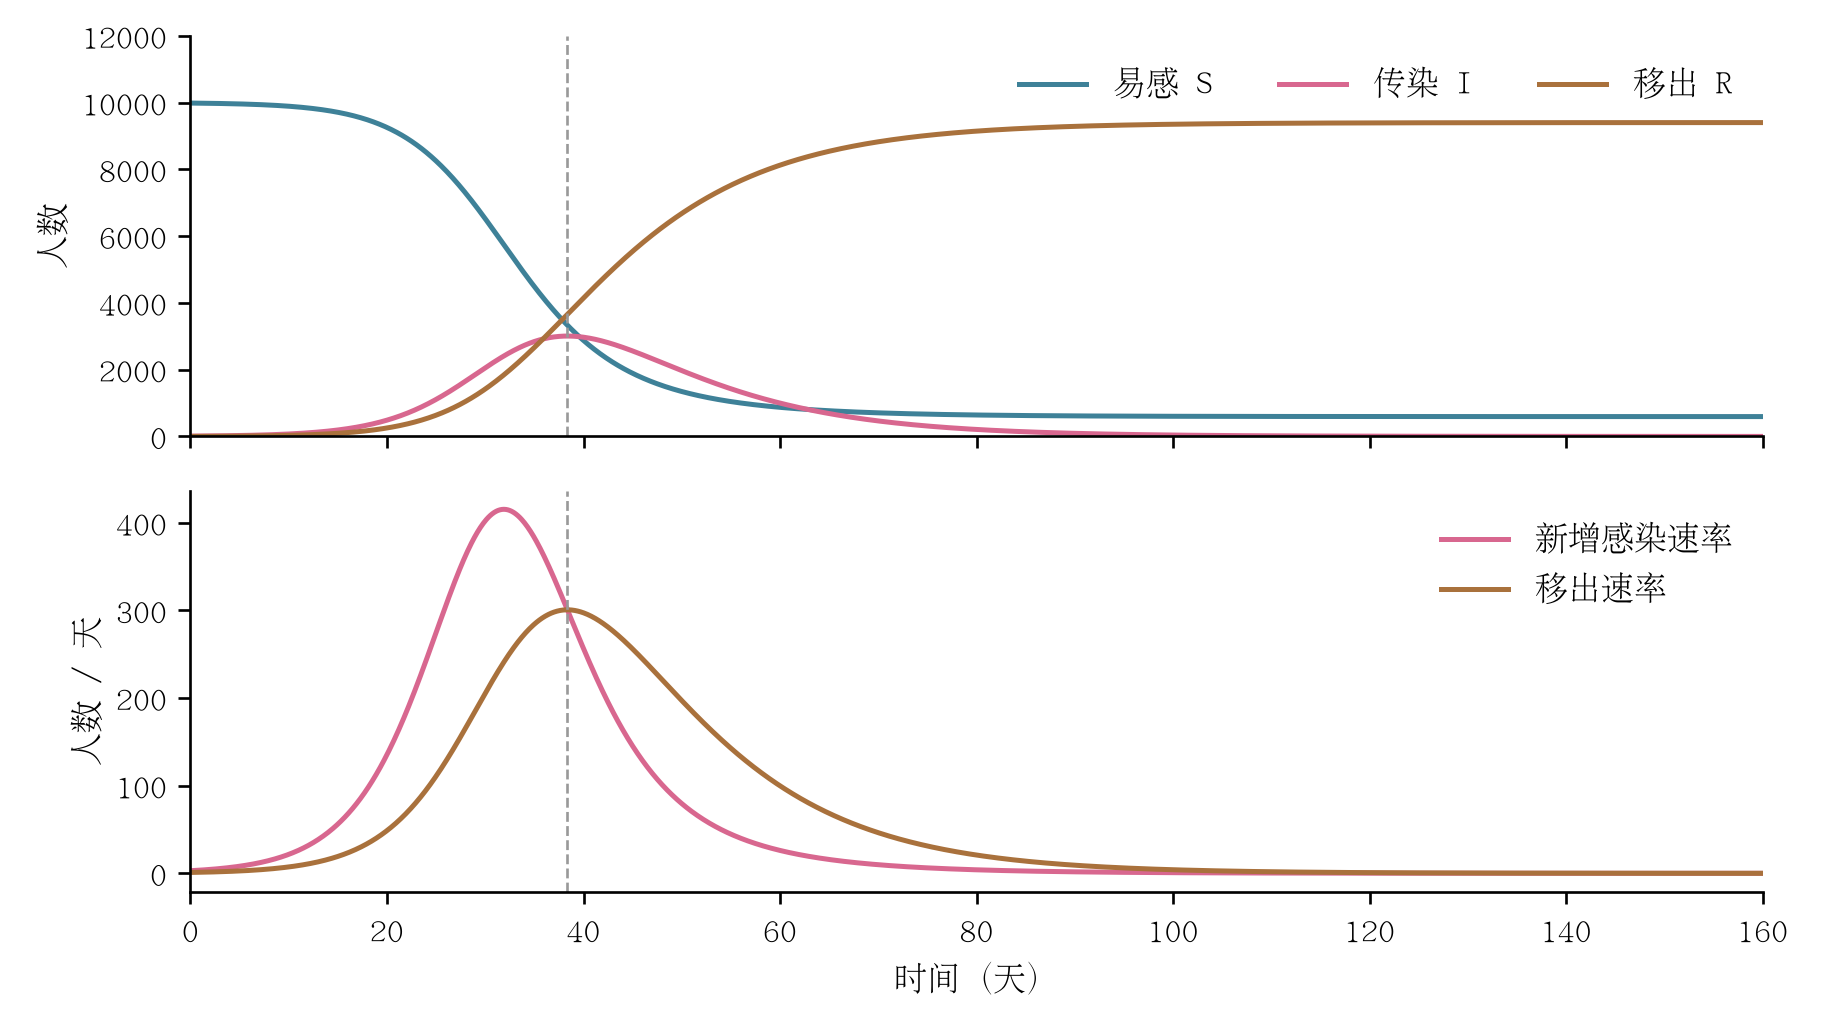
\includegraphics[width=0.94\linewidth]{images/sir_stocks_flows.png}

\small 上：三类人数，是存量。下：新增感染与移出速度，是流量。灰色虚线为 $I$ 的峰值时刻。
\end{center}
数值计算中，$I$ 的峰值约在第 \textbf{38.36 天}，约为 \textbf{3008 人}；
新增感染速度的峰值却在第 \textbf{31.89 天}。
水池里水最多，与水龙头进水最快，本来就不必同时发生。

若想检查后一结论：对新增感染速率 $C=\beta SI/N$ 求变化速度，可得
\[
\dot C=C\left[\beta(S-I)/N-\gamma\right].
\]
因此本例中，新增速度转折满足 $(S-I)/N=1/\mathcal R_0$，而不是 $S/N=1/\mathcal R_0$。
刚才的图比较的是模型新增\emph{感染}与现有\emph{传染者}，
实际每日确诊还涉及检测、报告延迟与统计口径，不能直接等同。

\subsection{可跳过的推导：最终有多少人从未感染}
在 $s,i>0$ 时，把 $\dot i$ 除以 $\dot s$，就把时间消掉了：
\[
\frac{\mathrm di}{\mathrm ds}=-1+\frac{1}{\mathcal R_0s}.
\]
积分得到轨道上的不变量
\[
\boxed{i+s-\frac1{\mathcal R_0}\ln s
=i(0)+s(0)-\frac1{\mathcal R_0}\ln s(0).}
\]
其中 $\ln$ 是自然对数。这句话的意思是：虽不能轻易直接写出 $i(t)$，
但某几个量组合起来，在整个过程中保持不变。

对本例，$r(0)=0$，所以 $i(0)+s(0)=1$。
疫情结束时 $i$ 趋于 $0$，最终易感比例 $s_\infty$ 满足
\[
\ln\frac{s_\infty}{s(0)}=-\mathcal R_0(1-s_\infty).
\]
它不便用普通四则运算直接解出，但可以数值求根。
本例得到 $s_\infty\approx0.05945$：约 \textbf{594 人始终未感染}，
曾经感染者总数约 \textbf{9406 人}，包含最初的十人。
这是给定假设和参数的数学结果，不是某个真实地区的预测。
也可看出：即使最高同时只有三千多人在 $I$ 中，累计经历过感染的人仍能多得多。

\section{改参数与改结构，是两件不同的事}
\subsection{降低传播参数，只改同一套方程里的一个数}
保持初值和 $\gamma$ 不变，把 $\beta$ 分别设为 $0.3,0.18,0.09$，
对应基本再生数为 $3,1.8,0.9$。
下面各条曲线都从初始时刻起使用各自固定参数，\emph{不是}在某一天突然切换措施的模拟。
\begin{center}
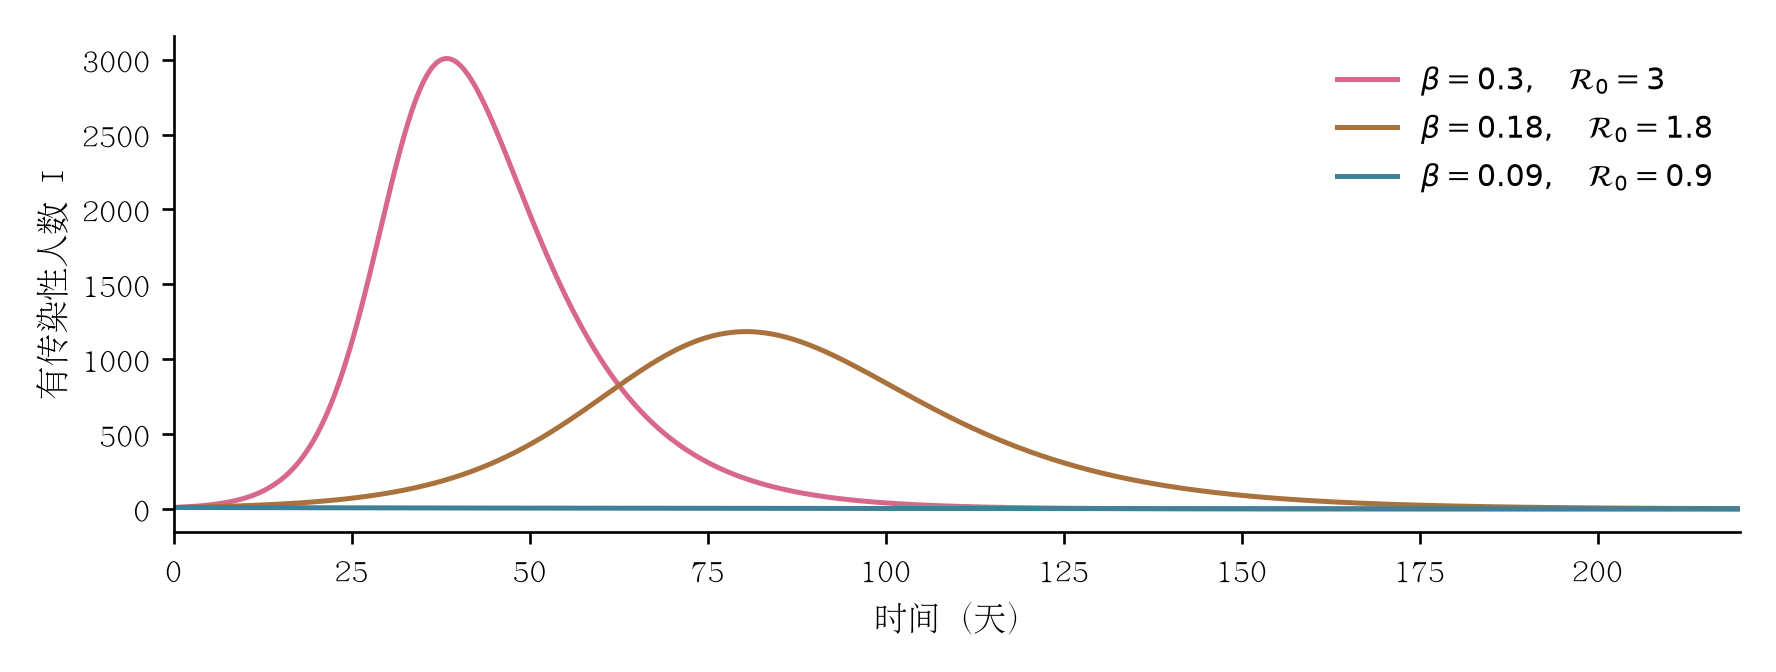
\includegraphics[width=0.91\linewidth]{images/sir_beta.png}

\small 其余条件相同，改变 $\beta$。参数较小的增长波峰较低、较晚；$\mathcal R_0=0.9$ 的例子从起点便下降。
\end{center}
若从一开始就有一部分人被完美且持续保护，且仍满足均匀混合等理想假设，
初始有效再生数会相应降低。
但 $\mathcal R_{\mathrm e}<1$ 的数学含义是\emph{此时 $I$ 在下降}，
并不表示不会再发生任何新增感染，也不自动给出实际干预方案。

\subsection{SIS、SEIR：改的是箭头，不只是调大小}
SIR 没有免疫衰减，也没有潜隐阶段。若问题需要，就必须改结构：
\begin{itemize}
\item \textbf{SIS}：移出传染状态后重新易感，箭头是 $S\to I\to S$。
在总人数固定时，$s=1-i$，于是
\[
\dot i=\beta(1-i)i-\gamma i=(\beta-\gamma)i-\beta i^2.
\]
当 $\beta>\gamma$ 时，这就是一种逻辑斯谛增长形式，正平衡为
$i_*=1-\gamma/\beta$；它可以长期保持非零的传染比例。
\item \textbf{SEIR}：加入已感染但尚无传染性的 $E$，箭头是
$S\to E\to I\to R$。若 $E$ 以速率 $\sigma$ 进入 $I$，则
$\dot E=\beta SI/N-\sigma E$，$\dot I=\sigma E-\gamma I$，其余两式相应保留。
这里 $E$ 对应无传染性的潜隐阶段，并不必然等于日常说的“尚未出现症状”。
\end{itemize}
若还要考虑免疫衰减、新生人口、季节变化或分组接触，基础 SIR 就不能原样照用。
尤其不能用一组固定参数的封闭 SIR 反复制造多轮波峰，却不解释新增的机制。

\section{先看全家福：LV 不只有捕食}
Lotka--Volterra（下文简称 LV）并不是只指“兔子与狐狸”那一对方程。
更一般的两种群形式是
\begin{equation}\label{eq:general-lv}
\boxed{\begin{aligned}
\dot X&=X(r_1+a_{11}X+a_{12}Y),\\
\dot Y&=Y(r_2+a_{21}X+a_{22}Y).
\end{aligned}}
\end{equation}
先读括号：它表示\textbf{平均到每个个体的增长速度}。
例如 $\dot X/X$ 是单位时间的相对增长率；乘回 $X$，才是整个种群的变化速度。
$r_1,r_2$ 是数量很少、没有另一物种影响时的内禀增长率，可以为正，也可以为负。
$a_{11}X,a_{22}Y$ 描述自身数量的影响，负系数常用来表达拥挤和资源限制。

真正区分相互作用类型的，是两个交叉系数：
$a_{12}$ 表示 $Y$ 对 $X$ 的影响，$a_{21}$ 表示 $X$ 对 $Y$ 的影响。
下标的顺序可以记成“后一个物种影响前一个物种”。
\begin{center}
\begin{tabular}{ccp{8.4cm}}
\toprule
$a_{12}$ & $a_{21}$ & 相互作用的含义\\\midrule
负 & 正 & 捕食：$X$ 受损，$Y$ 获益\\
负 & 负 & 竞争：双方都给对方的增长增加压力\\
正 & 正 & 互利合作：双方都提高对方的增长率\\\bottomrule
\end{tabular}
\end{center}
若交换捕食者与猎物的命名，捕食那一行的正负顺序也会交换。
某个系数为零，则表示模型中没有设置那个方向的直接作用。
这里的“合作”指种群层面的\textbf{互利}，不要求个体有合作意图。

\begin{warnbox}[正负号说的是影响，不是此刻数量的涨跌]
“竞争”不表示双方此刻都在减少，“互利”也不表示双方始终增加。
正负号描述的是：固定其他条件，另一物种增加会怎样改变本物种的\emph{相对增长率}。
此刻总的增长或减少，要看括号里所有项相加后的结果。
\end{warnbox}

接下来依次看捕食、竞争、互利三个版本。
每个版本都要说明自身增长与资源限制；不能只改一个交叉项的符号，就把前一版本的结论全部照搬。

\section{换一个舞台：兔子与狐狸为什么一多一少}
现在让 $X(t)$ 表示猎物数量，$Y(t)$ 表示捕食者数量。
用兔子和狐狸作比喻，但下面不是为真实兔狐数据拟合的模型。
这里取 Lotka--Volterra 家族中经典的两物种捕食者--猎物版本，写作
\begin{equation}\label{eq:lv}
\boxed{\begin{aligned}
\dot X&=aX-bXY,\\
\dot Y&=cXY-dY,
\end{aligned}\qquad a,b,c,d>0.}
\end{equation}
先逐项读：
\begin{itemize}
\item $aX$：没有捕食者时，猎物按指数规律增长；
\item $bXY$：相遇造成猎物损失，猎物与捕食者越多，捕食总量越大；
\item $cXY$：食物支持捕食者增长；它不是猎物变成捕食者的人数搬运；
\item $dY$：没有猎物时，捕食者按比例衰减。
\end{itemize}
若把每个被捕食猎物对捕食者增长的转换效率记为 $e$，可写 $c=eb$。
因此 $b$ 与 $c$ 不必相等，更不能要求捕食损失与捕食者增长在个体数上完全抵消。
$X+Y$ 一般不守恒：这不是把同一群人搬进不同仓室。

在以个体数为单位的写法中，$a,d$ 的单位是 $1/\text{时间}$，
$b$ 的单位为 $1/(\text{捕食者数}\cdot\text{时间})$，
$c$ 的单位为 $1/(\text{猎物数}\cdot\text{时间})$。
它们与前面带 $1/N$ 的 SIR 参数 $\beta$ 不能不加说明地共用同一组数字。

\begin{warnbox}[经典版本把什么省掉了]
没有捕食者，猎物可以无限指数增长；捕食者只有这一类食物；
每一对猎物与捕食者的相遇贡献相同，没有吃饱、躲藏、领地与年龄结构；环境和参数不随时间变化。
这些假设能让反馈结构看得很清楚，也正是它不能原封不动解释所有生态数据的原因。
\end{warnbox}

\section{不必先解方程，也能判断往哪个方向走}
将式 \eqref{eq:lv} 写成
\[
\dot X=X(a-bY),\qquad\dot Y=Y(cX-d).
\]
在 $X,Y>0$ 的区域里，增长方向由括号决定：
\[
\begin{array}{lll}
Y<a/b&\Rightarrow&\text{猎物增长},\\
Y>a/b&\Rightarrow&\text{猎物减少},\\
X>d/c&\Rightarrow&\text{捕食者增长},\\
X<d/c&\Rightarrow&\text{捕食者减少}.
\end{array}
\]
所以猎物能不能增长，要看捕食者有多少；捕食者能不能增长，则要看猎物有多少。
两条转折线交于\textbf{共存平衡点}
\[
\boxed{X_*=\frac dc,\qquad Y_*=\frac ab.}
\]
此外 $(0,0)$ 也是平衡。若初值严格为正，经典方程的解会一直保持为正，
并不会因为捕食者一多就自动在有限时间把某个种群变成恰好零。

\subsection{一个数值例子，和一次迟到的峰值}
取时间单位为年，假设
\[
a=1,\quad b=0.1,\quad c=0.02,\quad d=0.5,
\qquad X(0)=40,\quad Y(0)=9.
\]
此时 $X_*=25,Y_*=10$。
最开始，$\dot X=40(1-0.1\times9)=4>0$，
$\dot Y=9(0.02\times40-0.5)=2.7>0$，\textbf{两个种群会先一起增长}。
不是所有时刻都“一个增加，另一个必定减少”。

随着捕食者升到 $Y=10$，猎物先转为下降；
此时猎物仍多于 $25$，所以捕食者还能继续增加。
直到猎物跌到 $X=25$，捕食者才到达峰值。
随后捕食者减少，猎物面临的压力减轻，又有机会回升。
本例的第一次猎物峰约在第 $0.34$ 年，捕食者峰约在第 $2.18$ 年。
这种相位差由动力学产生，并不表示方程里显式放入了一个固定的“延迟几年”参数。

\begin{center}
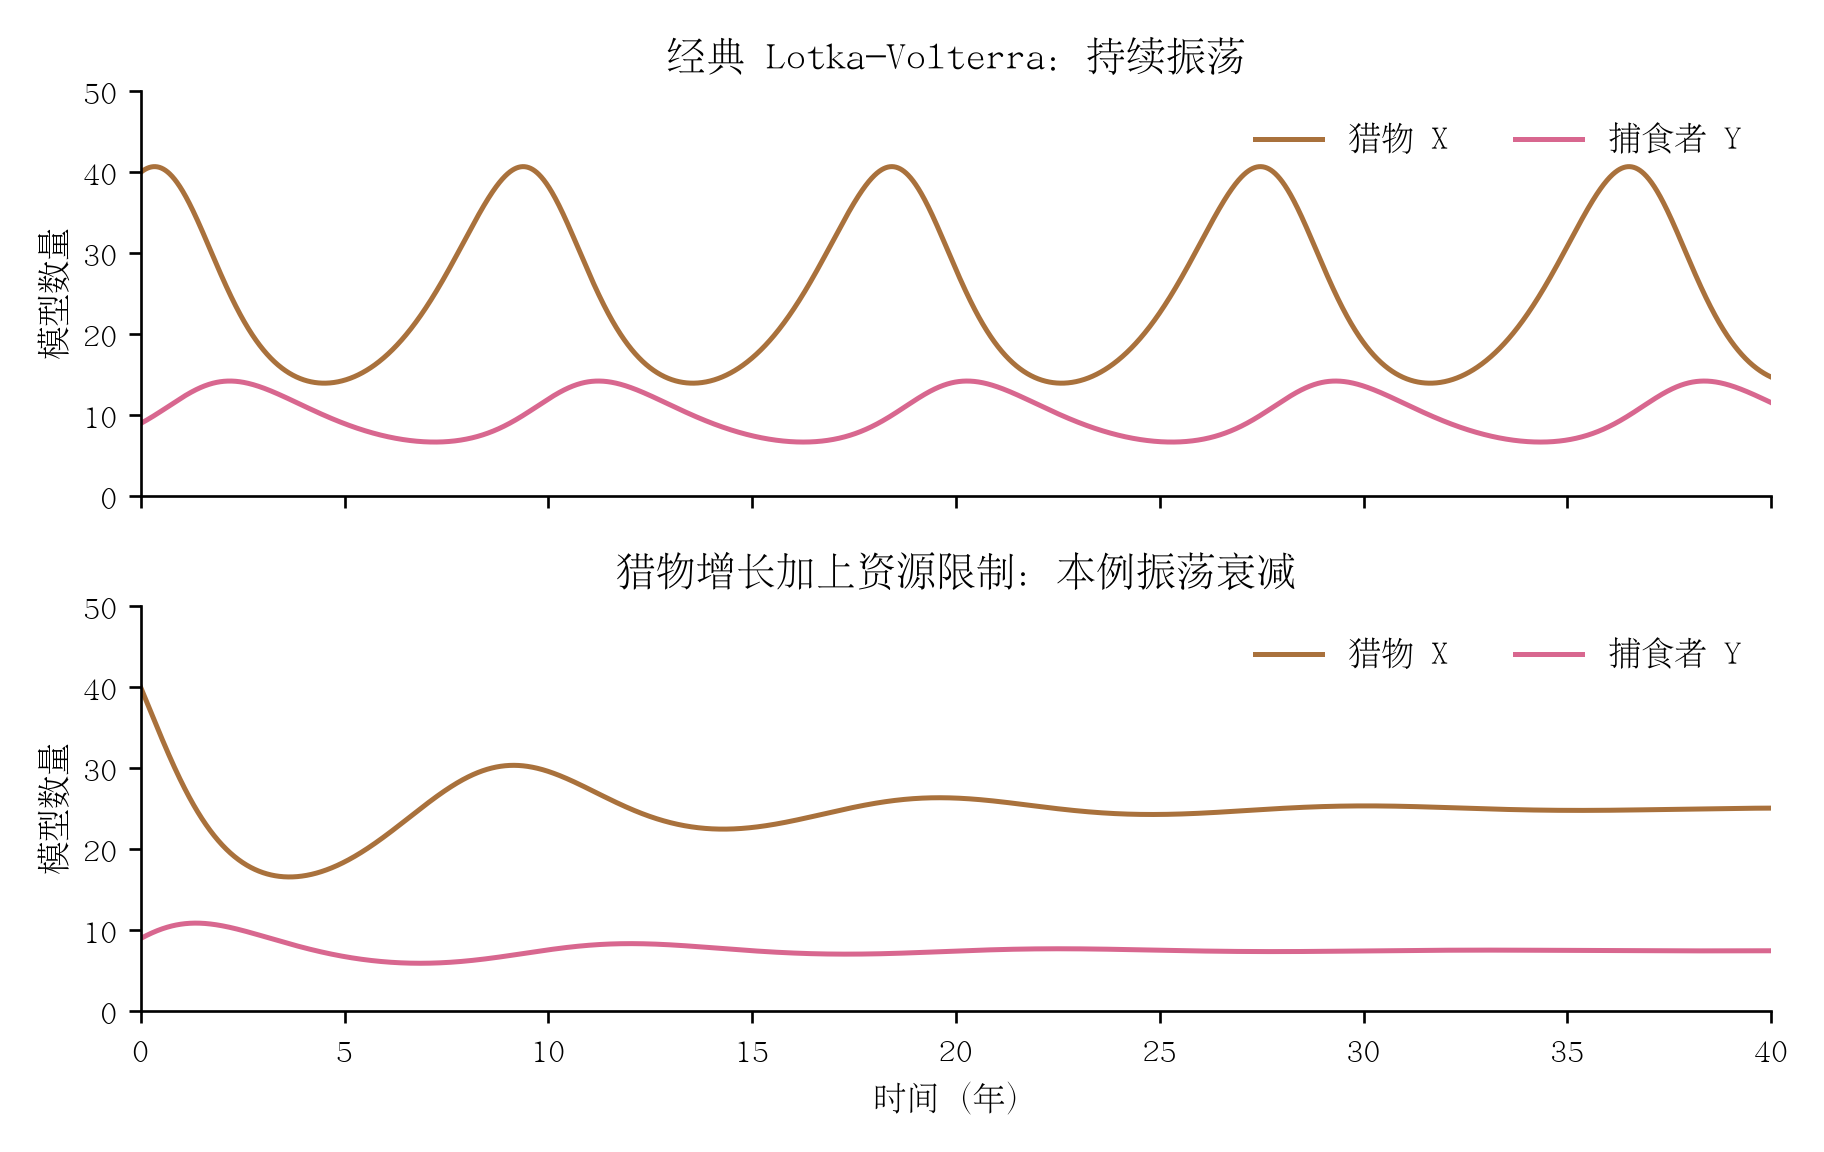
\includegraphics[width=0.94\linewidth]{images/lv_timeseries.png}

\small 上：经典模型。下：稍后介绍的资源受限版本；初值相同，但平衡位置也随模型改变。
\end{center}

\section{把时间藏起来：相图与闭合轨道}
时间曲线横轴为 $t$，一条画 $X$，一条画 $Y$。
\textbf{相图}则改用 $X$ 作横轴、$Y$ 作纵轴，
让同一时刻的两个数合起来成为一个点 $(X(t),Y(t))$。
时间往前走，这个点就沿一条\textbf{轨道}移动。

在相图上，竖线 $X=X_*$ 让 $\dot Y=0$，横线 $Y=Y_*$ 让 $\dot X=0$。
这类“某个变量暂时不增不减”的线叫\textbf{零增长线}，也叫零流线。
落在一条线上并不表示整个系统停住：只有两种变化速度\emph{同时}为零，才是平衡。

\begin{center}
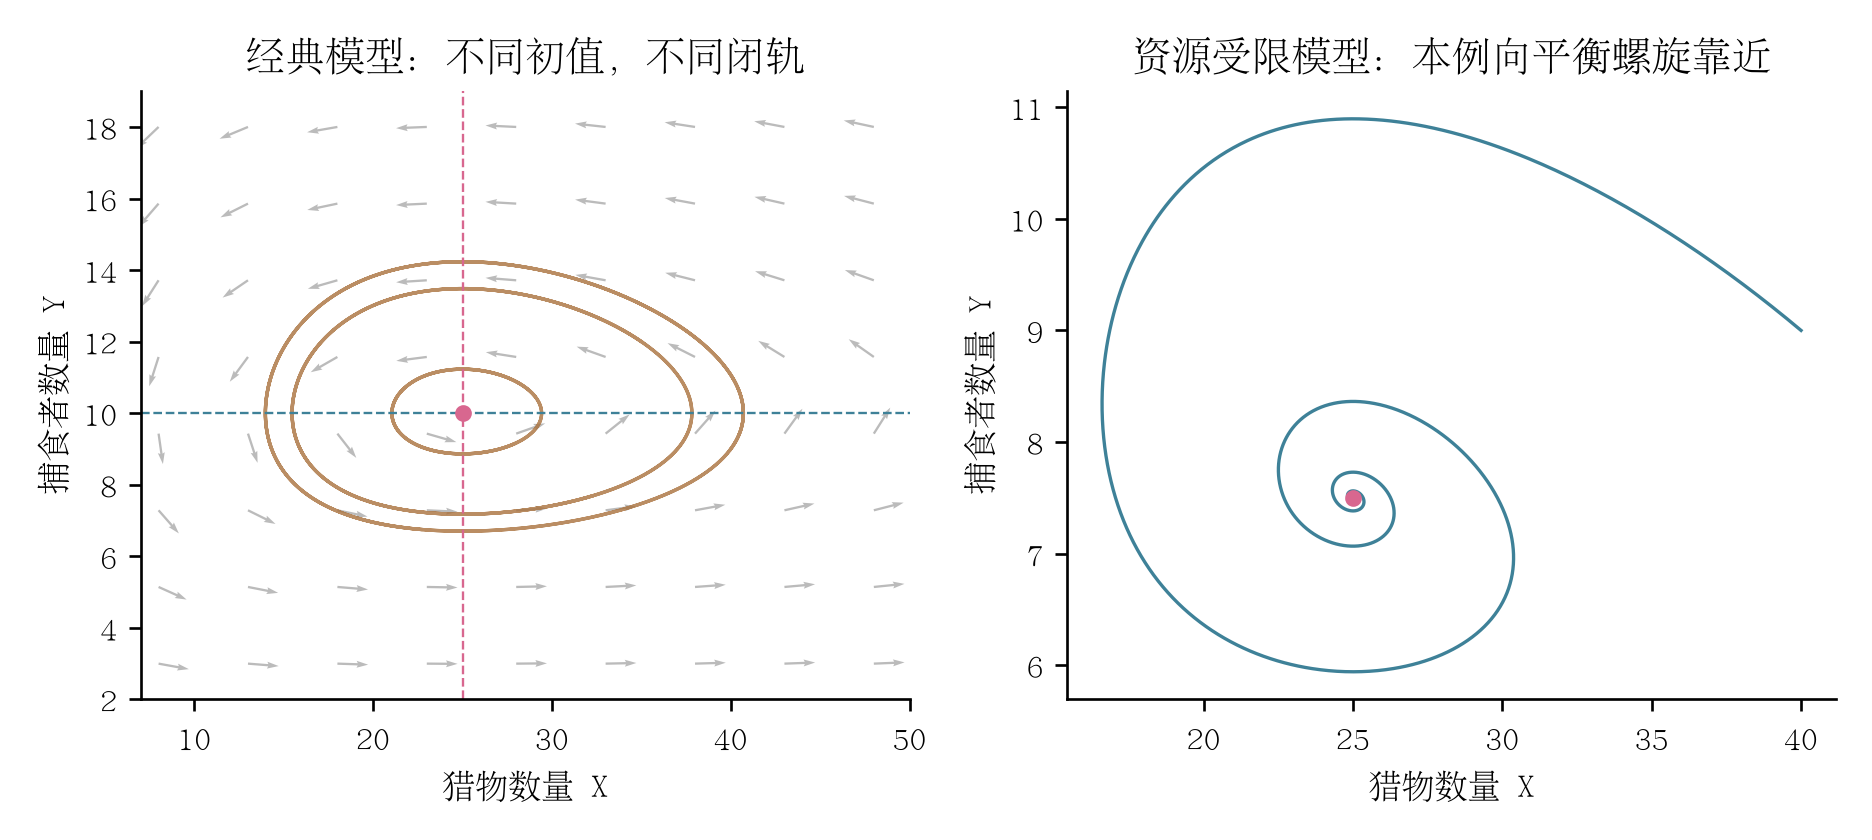
\includegraphics[width=0.96\linewidth]{images/lv_phase.png}

\small 左：经典模型的三组正初值，各沿不同闭合轨道运行，灰箭头表示运动方向。
右：资源受限的例子向新平衡点螺旋靠近。
\end{center}
经典模型里，每条正的非平衡轨道都围绕共存点闭合，因而对应周期振荡。
但这些轨道\textbf{不是一个吸引附近所有初值的极限环}：
换一个初值，通常就换一条闭合轨道，不会自己回到原先那一条。
共存点是一个中心，稳定于小扰动，但不是让附近轨道越绕越近的渐近稳定点。

\subsection{可跳过的计算：为什么轨道既不向里也不向外漂}
用平衡数量作尺度，定义 $u=X/X_*,v=Y/Y_*$，则
\[
\dot u=au(1-v),\qquad\dot v=dv(u-1).
\]
考虑一个组合量
\[
H=d(u-1-\ln u)+a(v-1-\ln v).
\]
它不是现实中的总个体数，也不必解释成物理能量。
对它求变化速度，用链式法则：
\begin{align*}
\dot H
&=d(1-1/u)\dot u+a(1-1/v)\dot v\\
&=ad(u-1)(1-v)+ad(v-1)(u-1)=0.
\end{align*}
所以每条轨道都保持自己的 $H$ 值。
函数 $z-1-\ln z$ 在 $z=1$ 时最小为零，偏向零或无限大时都会变大；
由此可进一步证明，正象限里 $H$ 的非零等值线是包围 $(1,1)$ 的闭曲线。
轨道既不能跨到别的 $H$ 值，也就不会慢慢向里收缩或向外扩散。

在平衡附近，若令 $u=1+\xi,v=1+\eta$ 并忽略小量乘积，得到
$\dot\xi\approx-a\eta,\dot\eta\approx d\xi$，
这与小振动的方程相同，近似周期为
\[
T_{\text{小振幅}}\approx\frac{2\pi}{\sqrt{ad}}.
\]
本例约为 $8.89$ 年。它是\emph{平衡附近}的近似；不能据此断言任意大振幅轨道都有相同周期。

\section{给猎物加上资源上限，图就会变}
如果读过逻辑斯谛增长模型，很自然会问：没有捕食者时，猎物为什么可以无限增长？
把它改为有承载量 $K$ 的增长，就得到
\[
\dot X=aX\left(1-\frac XK\right)-bXY,
\qquad\dot Y=cXY-dY.
\]
这是经典 Lotka--Volterra 的一个扩展，不应再把原模型的全部结论直接搬过来。
当 $K>d/c$ 时，共存平衡为
\[
X_*^{\text{新}}=\frac dc,\qquad
Y_*^{\text{新}}=\frac ab\left(1-\frac{d}{cK}\right)>0.
\]
若本例取 $K=100$，新平衡是 $(25,7.5)$，并非原来的 $(25,10)$。
前两张种群图的下半幅和右半幅，展示的就是这次改动。
所选初值下，振荡逐渐减弱并靠近平衡；经典闭轨不再保持。

若会看线性化矩阵，可以再核验一次：在新共存点处，
矩阵的迹是 $-aX_*/K<0$，行列式是 $bcX_*Y_*^{\text{新}}>0$，所以局部吸引。
本例还具有一对带负实部的复特征值，因此呈螺旋靠近。
不熟悉这些词也不影响读图：\textbf{资源反馈改变了“偏离以后会不会缩回来”这件事}。
更复杂的捕食饱和、时滞或季节项又可能产生其他行为，不能用一个例子概括所有扩展。

\section{竞争：争同一份资源，结局只有一方胜出吗}
想象两种植物占据同一片空间。即使没有另一种植物，自己太多也会拥挤；
另一种植物的增加，则会进一步挤占生长机会。一个常用的 LV 竞争模型是
\[
\dot X=r_1X\left(1-\frac{X+k_{12}Y}{K_1}\right),\qquad
\dot Y=r_2Y\left(1-\frac{Y+k_{21}X}{K_2}\right),
\]
其中 $r_1,r_2,K_1,K_2,k_{12},k_{21}$ 都为正。
$K_1,K_2$ 是各自\emph{单独存在时}的承载量。
$k_{12}Y$ 把第二物种造成的压力，折算成对第一物种而言相当于多少本物种个体；
$k_{21}X$ 同理。它们不要求相等。

\subsection{先统一刻度，再比较竞争强弱}
把数量换成各自承载量的倍数：$x=X/K_1,y=Y/K_2$。
于是单独生存时，各自的正平衡都变成 $1$，模型简化为
\begin{equation}\label{eq:competition}
\boxed{\dot x=r_1x(1-x-\alpha y),\qquad
\dot y=r_2y(1-y-\beta x),}
\end{equation}
其中 $\alpha=k_{12}K_2/K_1,\ \beta=k_{21}K_1/K_2$。
\textbf{本节的 $\beta$ 是竞争系数，与 SIR 的传播参数没有关系。}
$x=0.5$ 表示第一物种达到其单独承载量的一半，不是两个物种合起来的占比。

怎么看谁能留下来？设 $y$ 已经独自在 $y=1$ 附近生活，
这时引入一点点 $x$，它的相对增长率约为 $r_1(1-\alpha)$。
所以 $\alpha<1$ 时，稀少的 $x$ 可以增长；$\alpha>1$ 时则难以建立。
反过来，$x=1$ 附近稀少的 $y$ 能否增长，由 $\beta<1$ 决定。
这种“先看稀少的一方能否进入”的办法，不必先把方程全部解出来。

对于严格为正的初值，避开 $\alpha=1$ 或 $\beta=1$ 等临界情形，有四类结局：
\begin{center}
\small
\begin{tabular}{p{2.7cm}p{3.2cm}p{7.9cm}}
\toprule
参数范围 & 稀少的一方能否增长 & 典型长期结局\\\midrule
$\alpha<1,\beta<1$ & 双方都能 & 稳定共存；小扰动后能够返回\\
$\alpha<1,\beta>1$ & 只有 $x$ 能 & $x$ 留下，$y$ 渐近趋零\\
$\alpha>1,\beta<1$ & 只有 $y$ 能 & $y$ 留下，$x$ 渐近趋零\\
$\alpha>1,\beta>1$ & 双方都不能 & 两个边界结局都能吸引附近状态；胜负取决于初值\\\bottomrule
\end{tabular}
\end{center}
这里的“排斥”是连续模型里趋向零，不是说某一天最后一个个体必然消失。
最后一行通常叫\textbf{双稳态}：系统有两个可吸引附近状态的结局。
两个吸引区域之间还隔着一条特殊的分界轨道；恰好落在分界上的状态是例外。

\subsection{能算出正平衡，不代表它会吸引轨道}
令两个括号同时等于零，得到直线
$x+\alpha y=1$ 和 $\beta x+y=1$。
当 $1-\alpha\beta\ne0$ 时，交点为
\[
\boxed{x_* =\frac{1-\alpha}{1-\alpha\beta},\qquad
 y_* =\frac{1-\beta}{1-\alpha\beta}.}
\]
若 $\alpha=\beta=0.5$，平衡是 $(2/3,2/3)$，附近轨道会靠拢。
若 $\alpha=\beta=1.5$，也有正交点 $(0.4,0.4)$，却不是稳定共存：
偏向一边，可能最终留下 $x$；偏向另一边，则可能最终留下 $y$。
在图中 $r_1=r_2=1$ 的对称情形，直线 $x=y$ 正好就是分界。

\begin{center}
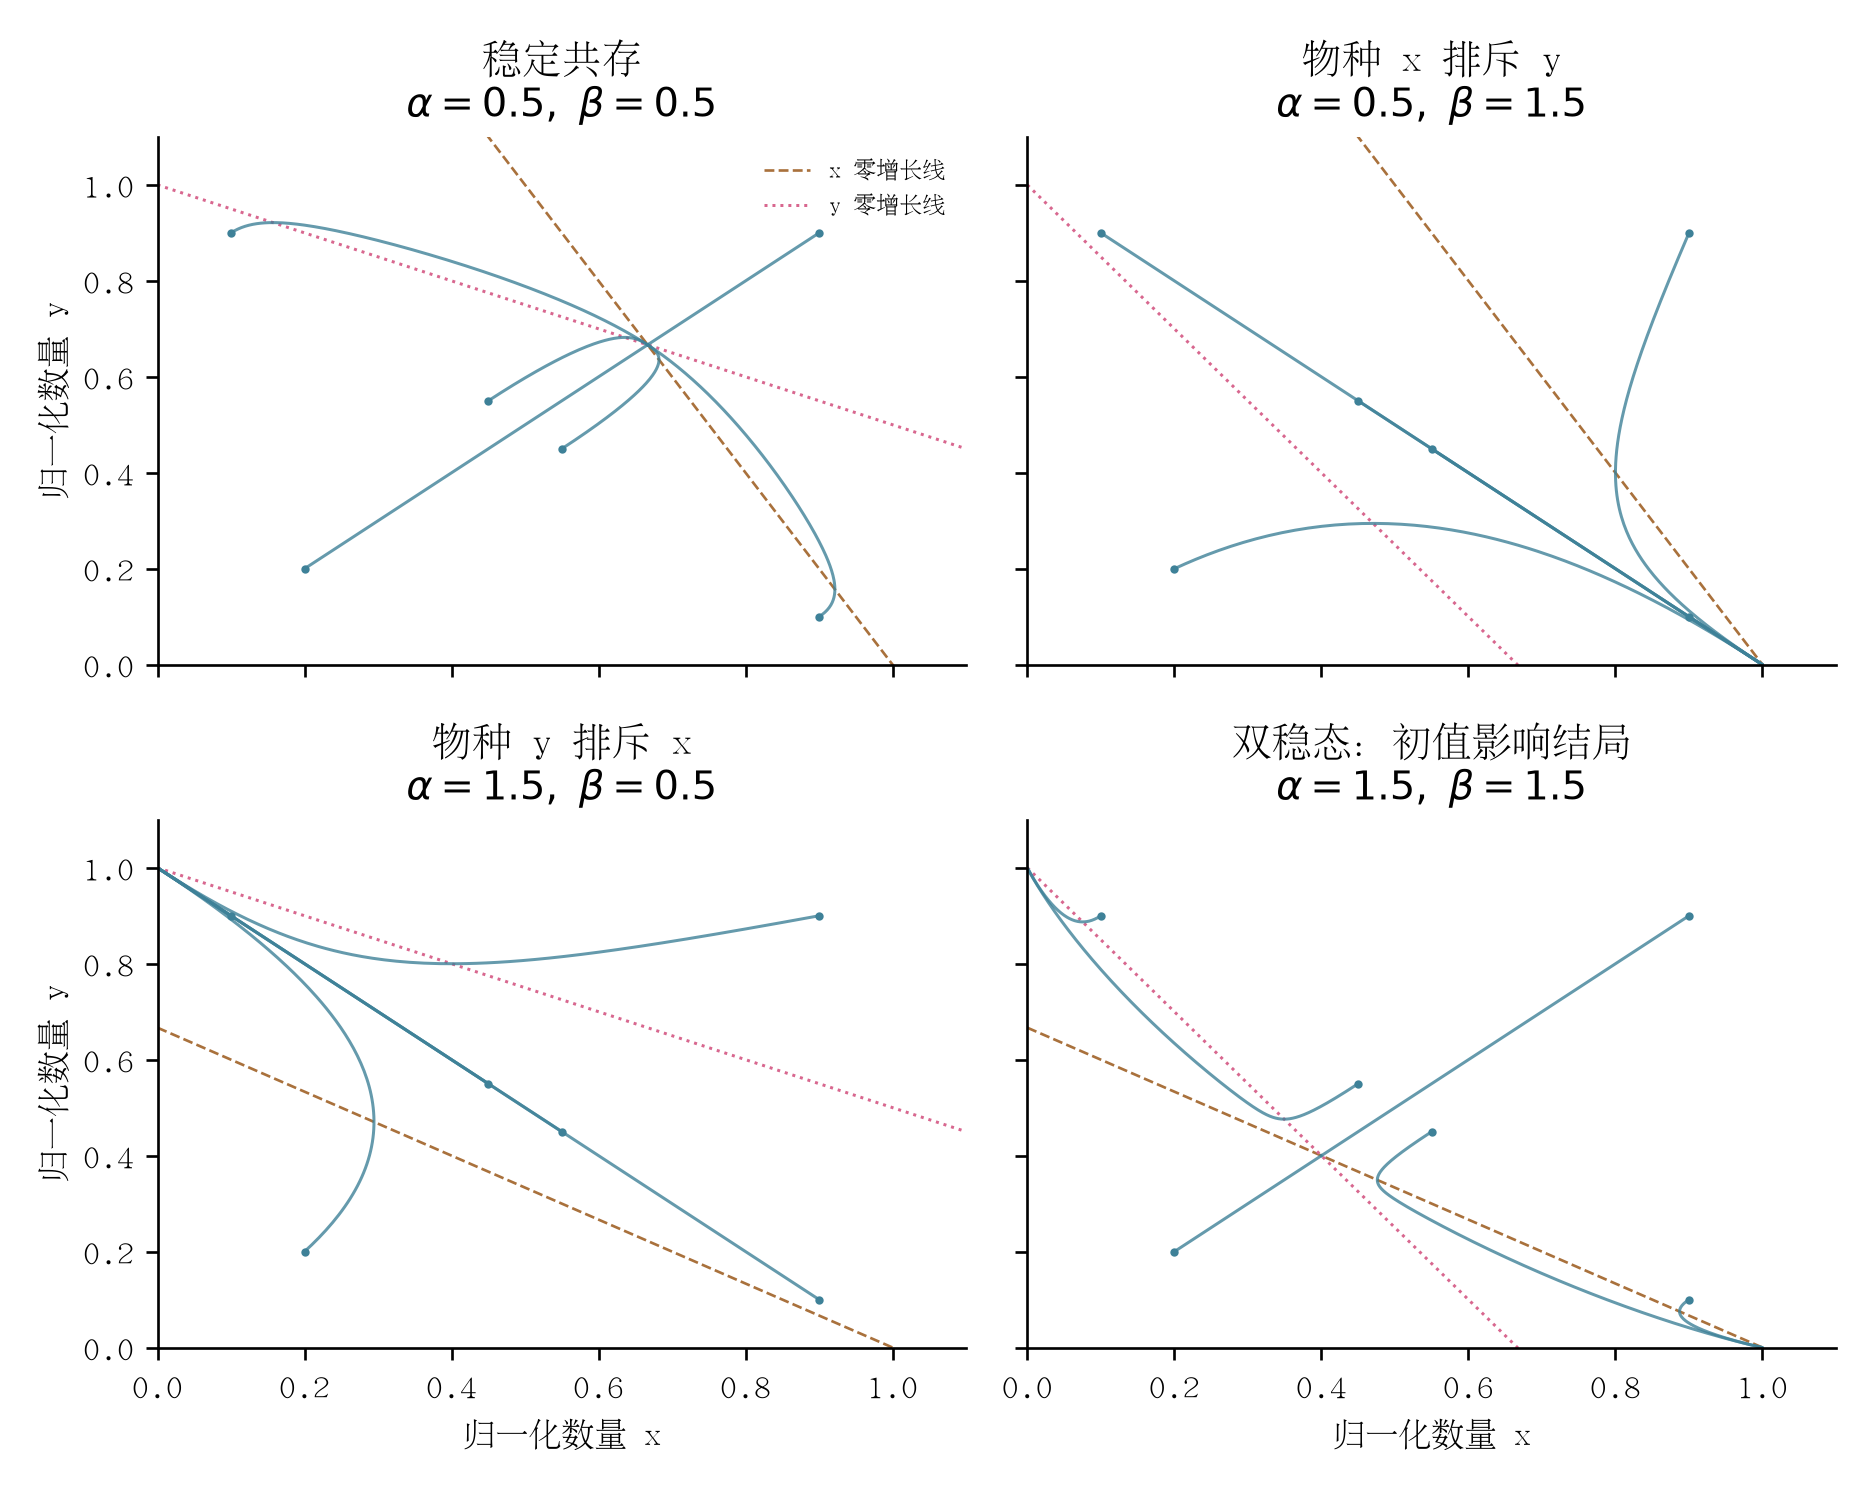
\includegraphics[width=0.93\linewidth]{images/competition.png}

\small 四组竞争强度，均取 $r_1=r_2=1$。蓝色圆点为初值，轨道向各自的长期结局移动。
虚线和点线是两条内部零增长线；右下图对角线上的特殊轨道趋向不稳定的内部平衡。
\end{center}

\begin{keybox}[为什么竞争也可能共存]
在这里，稳定共存需要归一化后的 $\alpha<1$、$\beta<1$：
双方对自己的限制，相比另一物种在其单独承载量时施加的限制，都足够强。
只检查乘积 $\alpha\beta<1$ 不够，例如 $0.5\times1.5<1$，却是 $x$ 排斥 $y$。
“有正平衡”“平衡稳定”“从某个初值会到哪里”是三个不同的问题。
\end{keybox}

\section{互利合作：帮助对方，也需要约束}
现在把竞争的负面作用改成正面作用，同时保留自身拥挤带来的限制：
\begin{equation}\label{eq:mutualism}
\boxed{\dot x=r_1x(1-x+\mu y),\qquad
\dot y=r_2y(1-y+\nu x),\qquad r_1,r_2,\mu,\nu>0.}
\end{equation}
$+\mu y$ 表示第二物种提高第一物种的相对增长率，$+\nu x$ 表示反向帮助。
例如一种生物为另一种提供营养，另一种改善前者的生存环境，可以启发这样的写法；
具体物种是否真的符合线性帮助，仍要由数据判断。

这个版本中，每一方独自也能生存，因此描述的是\textbf{非专性互利}。
如果离开伙伴便无法维持种群，就需要设置相应的负内禀增长率等机制，
属于\textbf{专性互利}的其他版本，不能直接套用下面的平衡公式。

\subsection{帮助适中：可以稳定在更高的数量}
两个括号同时为零，即 $x=1+\mu y,\ y=1+\nu x$。
当 $\mu\nu<1$ 时，得到正的共存平衡
\[
\boxed{x_* =\frac{1+\mu}{1-\mu\nu},\qquad
 y_* =\frac{1+\nu}{1-\mu\nu}.}
\]
例如 $\mu=0.4,\nu=0.3$，则 $(x_*,y_*)\approx(1.591,1.477)$。
取 $r_1=1,r_2=0.8$，从 $(0.2,0.3)$ 出发，图中的两个数量逐渐靠近这个平衡。
超过 $1$ 并不矛盾：$1$ 是\emph{单独生活时}的承载尺度，合作改变了增长条件。

可跳过的稳定性核验：在共存点，线性化矩阵的迹为
$-r_1x_*-r_2y_*<0$，行列式为
$r_1r_2x_*y_*(1-\mu\nu)>0$，所以这个平衡局部渐近稳定。
直观上，小扰动会逐渐消退；这里的互利正反馈还压不过自身限制。

\subsection{帮助过强：线性模型可能冲向无限大}
如果帮助的强度永远随伙伴数量线性增加，就可能形成越来越强的正反馈。
看一个能算清楚的例子：取 $r_1=r_2=1,\mu=\nu=1.2$，
并从 $x(0)=y(0)=0.2$ 出发。由于完全对称，两者始终相等，记为 $z(t)$，于是
\[
\dot z=z(1+0.2z),\qquad
z(t)=\frac{0.2e^t}{1-0.04(e^t-1)}.
\]
当 $t$ 从左侧逼近 $t_{\mathrm b}=\ln26\approx3.258$ 时，分母趋零，数量冲向无限大。
这叫\textbf{有限时间发散}。公式在 $t_{\mathrm b}$ 之后的代数值不再是原初值问题的种群解。
时间只是这个假想参数例子的单位，不能解释成真实生态系统的“三年爆炸”。

\begin{center}
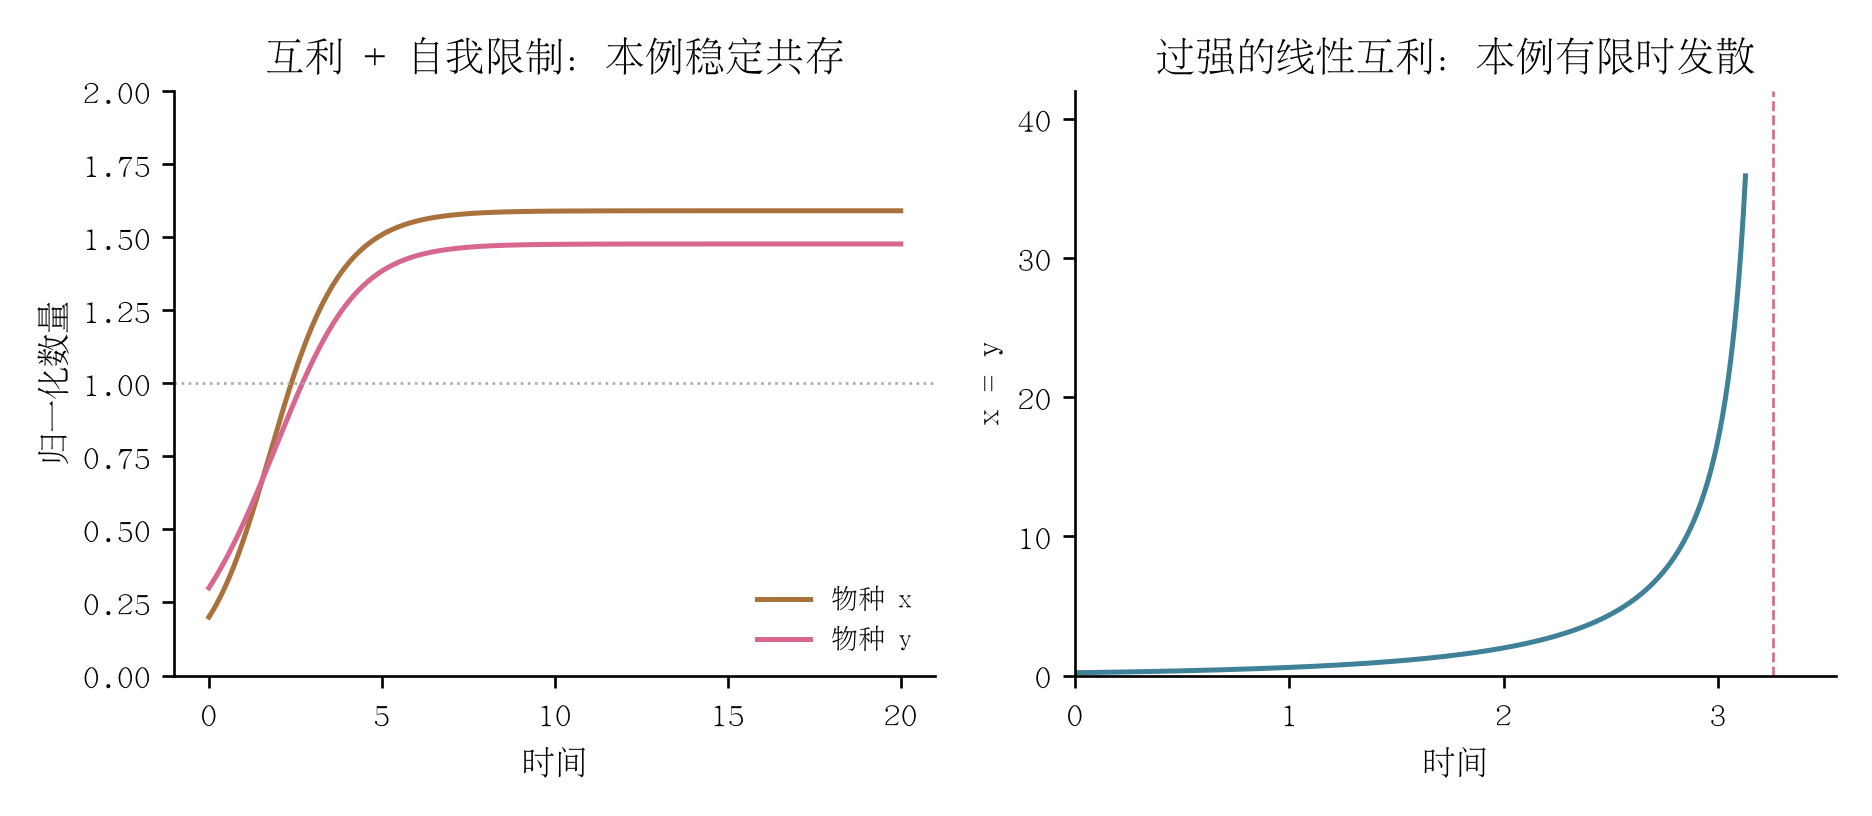
\includegraphics[width=0.96\linewidth]{images/mutualism.png}

\small 左：帮助适中，自身限制带来稳定共存。右：强互利的对称例子，竖虚线标出解析发散时间；
曲线在发散前停止绘制。两图参数不同，不能只比较曲线的高低。
\end{center}

这次发散可以从精确公式得到，并非电脑步长不够小。
它提醒我们：把局部适用的线性帮助无限外推，可能产生不合理的结局。
一种改法是让帮助\textbf{饱和}，例如把 $\mu y$ 换成
$\mu y/(1+hy)$，其中 $h>0$。当 $y$ 很大时，这个帮助项至多接近 $\mu/h$，
而自身限制 $-x$ 仍会增大。若双方都作相应改动，就能抑制这类无上限的正反馈。

\begin{warnbox}[合作的符号，不能代替完整的动力学分析]
互利既可能稳定共存，也可能在过度简化的方程里失控。
结果取决于自身限制、帮助强度、是否饱和、能否独立存活等具体假设。
捕食模型的闭合轨道也不是整个 LV 家族共有的性质。
\end{warnbox}

\section{再多几个物种：把关系装进矩阵}
生态系统通常不止两个物种。把前面的写法推广到 $n$ 个物种，就是
\[
\dot x_i=x_i\left(r_i+\sum_{j=1}^{n}a_{ij}x_j\right),\qquad i=1,\ldots,n.
\]
下标 $i$ 是物种编号，$\sum$ 表示把各物种的影响加起来。
例如三物种时，第一个括号就是 $r_1+a_{11}x_1+a_{12}x_2+a_{13}x_3$。
它仍然假设各种影响能按这些线性项相加；涉及“三者同时出现才产生作用”的高阶机制，需要另加模型项。

\subsection{矩阵不是新机制，而是一张有运算规则的关系表}
将数量和内禀增长率分别排成列向量，将系数排成矩阵：
\[
\mathbf x=\begin{pmatrix}x_1\\\vdots\\x_n\end{pmatrix},\qquad
\mathbf r=\begin{pmatrix}r_1\\\vdots\\r_n\end{pmatrix},\qquad
A=(a_{ij})_{n\times n}.
\]
矩阵第 $i$ 行、第 $j$ 列，记录的仍是“物种 $j$ 对物种 $i$ 的影响”。
$A\mathbf x$ 的第 $i$ 个分量，就是那一行系数分别乘数量后相加。
定义 $\operatorname{diag}(\mathbf x)$ 为主对角线上放 $x_1,\ldots,x_n$、其余位置全为零的矩阵，
它左乘一个向量，会把第 $i$ 个分量乘以 $x_i$。于是整组方程可写成
\[
\boxed{\dot{\mathbf x}=\operatorname{diag}(\mathbf x)(\mathbf r+A\mathbf x).}
\]
同一个 $A$ 可以同时含有捕食、竞争、互利关系，而且通常 $a_{ij}\ne a_{ji}$。
\textbf{矩阵表示让复杂关系更容易整理，却没有把原本的非线性微分方程变成线性方程。}

\subsection{第一件工具：用线性方程找全体共存的候选点}
若平衡点每个数量都严格为正，记为 $\mathbf x_*>0$，
那么每个括号都必须为零，故
\[
\boxed{A\mathbf x_*=-\mathbf r.}
\]
求平衡由此转化为解线性方程组！若 $A$ 可逆，唯一解为 $-A^{-1}\mathbf r$；
实际计算通常直接解方程，不必先算逆矩阵。
但\textbf{每个分量都为正}才是可行的全体共存平衡；出现负数，说明该候选点没有种群意义。
若 $A$ 不可逆，则要检查方程是否相容，可能无解，也可能有多个解，不能直接写逆矩阵。

\subsection{第二件工具：用特征值看小扰动会不会消退}
找到平衡后，把数量稍稍挪动，写成 $\mathbf x=\mathbf x_*+\mathbf u$。
代回方程，忽略扰动之间的乘积，得到近似
\[
\dot{\mathbf u}\approx J_*\mathbf u,\qquad
\boxed{J_*=\operatorname{diag}(\mathbf x_*)A.}
\]
$J_*$ 叫平衡处的\textbf{雅可比矩阵}，记录小变化如何影响变化速度。
一般不能直接用 $A$ 代替它：左边的对角矩阵给 $A$ 的各行乘上了不同的平衡数量。

对实特征向量 $\mathbf v$，若 $J_*\mathbf v=\lambda\mathbf v$，
则沿这个方向的线性扰动按 $e^{\lambda t}$ 缩小或放大。
这就是\textbf{特征值} $\lambda$ 与\textbf{特征向量} $\mathbf v$ 的用处。
特征值也可能是复数，虚部与振荡有关，判断衰减还是增长则看实部：
\begin{itemize}
\item 全部特征值的实部严格小于零：这个共存平衡局部渐近稳定；
\item 至少一个实部严格大于零：这个内部平衡不稳定；
\item 没有正实部，但有零实部：线性化不能直接定论，需要进一步分析。
\end{itemize}
前面经典捕食版本的纯虚特征值，就属于最后一种情况；
我们还借助不变量，才确认其闭合轨道。局部稳定也不等于任意远处的初值都会回到这里。

\subsection{一个能手算的三物种竞争例子}
取 $\mathbf r=(1,1,1)^{\mathsf T}$，上标 $\mathsf T$ 表示把一行转成一列，并设
\[
A=\begin{pmatrix}
-1&-0.2&-0.2\\
-0.2&-1&-0.2\\
-0.2&-0.2&-1
\end{pmatrix}.
\]
即三种群均有自身限制，任意另一个物种带来的竞争系数为 $0.2$。
由对称性，令三个平衡数量都为 $q$，则 $1-1.4q=0$，所以
\[
\mathbf x_*=\begin{pmatrix}5/7\\5/7\\5/7\end{pmatrix}>0,\qquad J_*=\frac57 A.
\]
$J_*$ 的特征值为 $-1,-4/7,-4/7$，全部为负，故该共存平衡局部渐近稳定。
例如 $(1,1,1)^{\mathsf T}$ 是特征值 $-1$ 的方向，表示三者一起偏多或偏少的扰动会消退；
$(1,-1,0)^{\mathsf T}$ 是特征值 $-4/7$ 的方向，表示一多一少的失衡也会消退。
用 NumPy 可以核验：
\Needspace{10\baselineskip}
\begin{lstlisting}
import numpy as np
A = np.array([[-1, -.2, -.2], [-.2, -1, -.2], [-.2, -.2, -1]])
r = np.ones(3)
x_star = np.linalg.solve(A, -r)
J = np.diag(x_star) @ A
print(x_star)             # [0.71428571, 0.71428571, 0.71428571]
print(np.linalg.eigvals(J))  # -1, -4/7, -4/7 (order may vary)
\end{lstlisting}

\begin{keybox}[三个问题，按顺序回答]
先问线性方程有没有解，再问候选数量是否全为正，最后问雅可比矩阵的特征值是否支持局部稳定。
对某些物种数量为零的边界平衡，不能把全部括号都设为零，也不能直接套用上面的简化雅可比公式。
尤其要检查消失物种在稀少时能否增长：其增长率为 $r_i+\sum_j a_{ij}x_j^*$，
这正是竞争一节中“稀少的一方能否进入”的多物种版本。
\end{keybox}

\section{回到传染病：同样是相遇，为何结局不同}
先把 SIR 与经典捕食版本作比较：
\begin{center}
\small
\begin{tabular}{p{2.6cm}p{5.7cm}p{5.7cm}}
\toprule
问题 & 封闭、常参数 SIR & 经典捕食者--猎物模型\\\midrule
变量是什么 & 同一群人的不同传播状态 & 两个不同种群的数量\\
相遇带来什么 & 易感者进入传染状态 & 猎物损失，支持捕食者增长\\
个体总数守恒吗 & $S+I+R=N$ 守恒 & $X+Y$ 一般不守恒\\
谁会自行补充 & 易感者不再补充 & 猎物在无捕食时会增长\\
典型长期行为 & 传染比例趋零，部分人仍易感 & 正的非平衡轨道周期振荡\\
相图中的障碍 & $S$ 单调减少，不能闭合循环 & 组合量 $H$ 守恒，形成闭轨\\\bottomrule
\end{tabular}
\end{center}
这张表先回答了文章开头的一个问题：两边都出现乘积项，并不代表会出现相同形状的曲线。

在基础 SIR 中，只要 $S,I>0$，就有 $\dot S<0$；
状态不可能绕一圈后回到原来的 $S$，所以没有非平凡的闭合周期轨道。
并且 $\mathcal R_{\mathrm e}$ 随 $S$ 单调下降，$I$ 至多由增长转为下降一次。
若一开始就低于阈值，则连先增长这一段也没有。

经典捕食者--猎物模型则有持续的反馈回路：
猎物能繁殖，捕食者靠猎物得到支持，捕食压力又反过来限制猎物，随后压力减小。
这不是人从 $S$ 经过 $I$ 最终留在 $R$ 的单向旅程。
竞争与互利又展示了其他结局：归一化后的竞争强度决定共存、排斥或双稳态；
互利能抬高稳定数量，也可能在帮助无上限的简化模型中导致发散。
\textbf{决定结论的，不只是某个乘法符号，而是整套流动、补充与反馈结构。}

\section{电脑也会画错：别把数值漂移当生态规律}
实际计算时，我们用足够小的时间步长，近似追踪微分方程。
最简单的显式欧拉法是
\[
X_{n+1}=X_n+h(aX_n-bX_nY_n),\qquad
Y_{n+1}=Y_n+h(cX_nY_n-dY_n),
\]
其中 $h$ 是步长，$n$ 标出计算步，真实时间为 $t_n=nh$。
它不是原微分方程的精确解，即使公式看起来很直接，也会积累误差。
\begin{center}
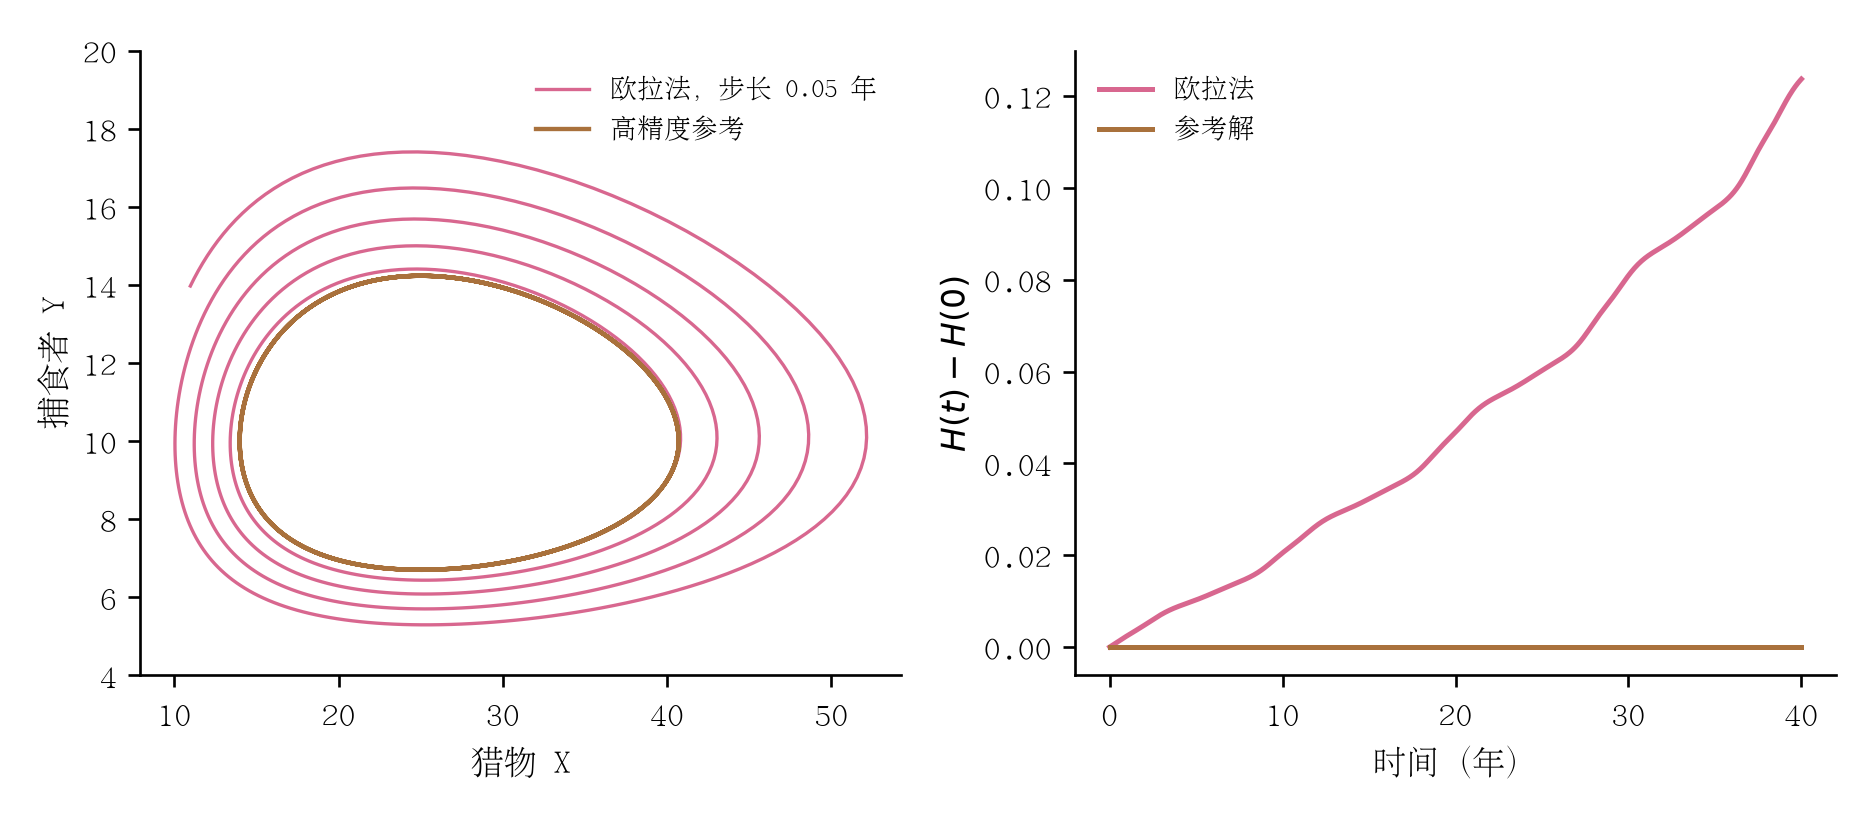
\includegraphics[width=0.96\linewidth]{images/numerical_drift.png}

\small 同一经典模型与初值。欧拉步长取 $0.05$ 年；左图的外漂伴随右图不变量的漂移。
参考解使用高精度自适应积分，未对轨道强行作闭合处理。
\end{center}
原模型的 $H$ 严格不变，欧拉法却可能使它逐步增加，画出向外的螺旋。
这时“振幅越来越大”首先是数值方法的信号，不能直接当成生态机制。
在 SIR 中，粗糙数值计算还可能给出负人数；事后把负数截成零会掩盖问题。

随文的 \texttt{数值实验.py} 用 NumPy、SciPy 和 Matplotlib 生成七张图，
并检查 SIR 总量守恒、峰值条件、最终规模方程、捕食版本的平衡与不变量，
以及竞争的四类结局、互利共存平衡、强互利的解析例子，
并核验三物种竞争例子的线性方程、雅可比矩阵与特征值；
还用更严格的积分精度比较结果。验证数据保存在 \texttt{验证数据.json} 中。
图中文字采用 TeX Live 自带文鼎宋体，其他机器可通过 \texttt{CJK\_FONT} 指定字体文件。
图像来自假想参数下的计算，没有把真实疫情或生态观测伪装成模拟结果。

\begin{keybox}[读完后，可以自己做的五个小检查]
\begin{enumerate}
\item 如果 $\mathcal R_0=3$，但易感者只占四分之一，此刻 $I$ 增还是减？
有效再生数为 $3/4<1$，所以在 $I>0$ 时下降，并不代表新增感染立即变成零。
\item 本例中若 $X=40,Y=12$，谁增谁减？
$Y>10$，猎物减少；$X>25$，捕食者仍增加。
\item 如果经典模型的相图越绕越外，先检查什么？
先检查 $H$ 的数值漂移与步长收敛，再判断是不是确实改变了原模型。
\item 竞争模型算出了正的内部平衡，是否就证明稳定共存？
没有。$\alpha=\beta=1.5$ 的内部平衡也为正，却不能吸引附近的一般初值。
\item 互利模型中的数量超过 $1$，是否一定算错了？
不一定。这里 $1$ 是单独生活时的承载尺度；应进一步检查增长是否有界、帮助机制是否合理。
\end{enumerate}
\end{keybox}

\Needspace{28\baselineskip}
\begin{keybox}[参考与继续阅读]
\begin{itemize}
\item W.~O.~Kermack, A.~G.~McKendrick，
\href{https://doi.org/10.1098/rspa.1927.0118}{A Contribution to the Mathematical Theory of Epidemics}，
\textit{Proceedings of the Royal Society A} \textbf{115}（1927），700--721。
早期传染病动力学的经典文献；本文介绍的是其研究路线下常用的简化 SIR 版本。
\item D.~Smith, L.~Moore，
\href{https://sites.math.duke.edu/education/ccp/materials/diffcalc/sir/}{The SIR Model for Spread of Disease}，
Duke University 教学材料。可对照仓室模型与易感比例、传染比例之间的关系。
\item \href{https://users.ssc.wisc.edu/~jdmontgomery/predatorprey.pdf}{Predator-Prey Models}，
University of Wisconsin--Madison 课程讲义，第 17 章。讨论经典模型、资源限制与数值迭代的差别。
\item \href{https://www.uwyo.edu/dbmcd/popecol/marlects/lect21.html}{Competition: Lotka--Volterra Model}，
University of Wyoming 种群生态学课程材料。可对照竞争的四类结局与零增长线。
\item W.~G.~Graves, B.~B.~Peckham, J.~Pastor，
\href{https://www.d.umn.edu/~bpeckham/export/Papers/GPP_UMD_TR2006-2.pdf}{A 2D Differential Equations Model for Mutualism}，
University of Minnesota Duluth 技术报告 TR 2006-2。
讨论非专性与专性互利，以及使帮助作用饱和的建模方法。
\item V.~Dobrushkin，
\href{https://www.cfm.brown.edu/people/dobrush/am34/Mathematica/ch3/linear.html}{Linearization}，
Brown University 微分方程教程。可继续阅读雅可比矩阵、特征值与局部稳定性。
\end{itemize}
\end{keybox}
\end{document}
